\chapter{Matroidy}

\section{Definícia, základné pojmy}

\begin{definition}
\label{def:matroid}
Dvojica $(X, \mathcal{N})$, kde $\mathcal{N} \subseteq \powerset(X)$ a $\mathcal{N}$ je konečná, je matroid, ak sú splnené nasledujúce podmienky:
\begin{enumerate}
    \item $\varnothing \in \mathcal{N}$
    \item $N \in \mathcal{N} \wedge N' \subseteq N \Longrightarrow N' \in \mathcal{N}$
    \item $N, N' \in \mathcal{N} \wedge \ssize{N} < \ssize{N'} \Longrightarrow \exists x \in N' - N: N \cup \set{x} \in \mathcal{N}$
\end{enumerate}

Množiny z $\mathcal{N}$ voláme nezávislé množiny. Množiny mimo $\mathcal{N}$ voláme závislé.
\end{definition}

\begin{theorem}{(Matroid z vektorového priestoru)}\\
Nech $V_n(F) \cong F^n$ je vektorový priestor dimenzie $n < \infty$ nad (nie nutné konečným) poľom $F$.
Nech $(\vec{x}_1, \ldots, \vec{x}_r)$ je postupnosť (nie nutné rôznych) vektorov z $V_n(F)$.
Nech $X := \set{1, \ldots, r}$, $\mathcal{N} := \set{Q ~|~ Q \subseteq X \wedge \set{\vec{x}_i ~|~ i \in Q} \text{ je nezávislá v } V_n(F) }$.
Potom dvojica $(X, \mathcal{N})$ je matroid.
\end{theorem}
\begin{proof}
Treba postupne overiť všetky tri podmienky z definície matroidu.
\paragraph{$\varnothing \in \mathcal{N}$:} Prázdna množina vektorov je (lineárne) nezávislá, takže patrí do množiny $\mathcal{N}$.
\paragraph{$N \in \mathcal{N} \wedge N' \subseteq N \Longrightarrow N' \in \mathcal{N}$:} Podmnožina (lineárne) nezávislej množiny vektorov je tiež (lineárne) nezávislá.
\paragraph{$N, N' \in \mathcal{N} \wedge \ssize{N} < \ssize{N'} \Longrightarrow \exists x \in N' - N: N \cup \set{x} \in \mathcal{N}$:} 
Sporom, nech $\forall x \in N' - N: N \cup \set{x} \notin \mathcal{N}$, čiže množina vektorov $N \cup \set{x}$ je vždy (lineárne) závislá. 
Potom platí, že vektor $x$ sa dá vyjadriť ako lineárna kombinácia zvyšných vektorov v tejto množine.
To znamená, že každý vektor z $N' - N$ sa dá vyjadriť ako lineárna kombinácia vektorov z $N$.

Z toho vyplýva, že dimenzia lineárneho obalu množiny $N'$ nie je väčšia ako dimenzia lineárneho obalu množiny $N$.
Nakoľko obidve množiny $N$ a $N'$ sú (lineárne) nezávislé, tak ich mohutnosti sú rovné dimenziám príslušných lineárnych obalov.
Potom $|N| \geq |N'|$, čo je spor.
\end{proof}

\begin{theorem}{(Matroid z grafu)}\\
\label{th:m_graph}
Nech $G = (V, E)$ je jednoduchý graf. Nech $X := E$. Nech množina hrán $A \subseteq E$ patrí do množiny $\mathcal{N}$ práve vtedy, keď
indukovaný graf neobsahuje kružnice. Potom dvojica $M(G) = (X, \mathcal{N})$ je matroid.
\end{theorem}
\begin{proof}
Schéma dôkazu je totožná s predošlou vetou, ponechávame preto tento dôkaz ako samostatné cvičenie (úloha \ref{ex:m_graph}).
\end{proof}

\begin{exercise}
\label{ex:m_graph}
Dokážte vetu \ref{th:m_graph}.
\end{exercise}

\begin{definition}
Nech $M = (X, \mathcal{N})$ je matroid a nech $A \subseteq X$. Množinu $B \subseteq A$ voláme bázou množiny $A$ v matroide $M$, ak 
je to maximálna (na inklúziu) nezávislá množina v $A$. Formálne, $B$ je bázou $A$ v matroide $M=(X, \mathcal{N})$, ak:
$$B \subseteq A \wedge B \in \mathcal{N} \wedge \left( \forall B' \supset B: B' \subseteq A \Longrightarrow B' \not\in\mathcal{N} \right)$$

Špeciálne, bázy množiny $X$ voláme bázy matroidu. Množinu báz matroidu $M$ znáčime ako $\mathcal{B}$.
\end{definition}

\begin{theorem}
Nech $(X, \mathcal{N})$ je matroid a $A \subseteq X$. Nech $N, N'$ sú bázy množiny $A$. Potom $\ssize{N} = \ssize{N'}$.
\end{theorem}
\begin{proof}
Sporom, nech mohutnosti báz $N$ a $N'$ sú rôzne.
BUNV, $|N| < |N'|$.
Potom z tretej vlastnosti matroidov (definícia \ref{def:matroid}) vyplýva, že existuje prvok $x \in N' - N \subseteq A$ taký, že $N \cup \set{x} \in \mathcal{N}$.
To je však spor s tvrdením, že množina $N$ je bázou, t.j. maximálnou na inklúziu nezávislou podmnožinou $A$.
\end{proof}

\begin{definition}
Nech $(X, \mathcal{N})$ je matroid. Hodnosťou množiny $A \subseteq X$ voláme veľkosť nejakej bázy $B$ množiny $A$ a znáčime ako $r(A) := \ssize{B}$.
\end{definition}

\begin{theorem}
\label{th:m_r}
Nech $(X, \mathcal{N})$ je matroid a $r:\powerset(X) \to \mathbb{N}_0$ je jeho hodnostná funkcia. Potom platí:
\begin{enumerate}
    \item $r(\varnothing) = 0$
    \item $r(\set{x}) \leq 1$
    \item $A \subseteq B \Longrightarrow r(A) \leq r(B)$
    \item $r(A \cup B) \leq r(A) + r(B) - r(A \cap B)$ (semimodularita)
\end{enumerate}

Navyše, ak nejaká funkcia $r':\powerset(X)\to\mathbb{N}_0$ spĺňa vyššie uvedené podmienky, tak existuje jediný matroid, ktorého
hodnostnou funkciou je práve $r'$.
\end{theorem}
\begin{proof}
% dokaz je prevzaty z https://sites.math.washington.edu/~morrow/336_09/papers/Will.pdf 
Prvé tri vlastnosti hodnostnej funkcie sú triviálne na dokazovanie, sústrediť sa budeme na štvrtú vlastnosť.

Nech $I$ je bázou množiny $A\cap B$.
Nech $I' \supseteq I$ je bázou množiny $A \cup B$, obsahujúca množinu $I$ (pomocou tretej vlastnosti\footnote{túto techniku budeme použivať aj neskôr} z definície matroidov).
Keďže každá podmnožina nezávislej množiny musí byť tiež nezávislá (druhá vlastnosť z definície matroidov), tak $|I' \cap (A \cap B)| \leq |I|$ (keďže $I$ je maximálna nezávislá množina v $A\cap B$). Keďže $I'$ (z definície) obsahuje $I$, tak platí $I' \cap (A \cap B) = I$. 

Ďalej platí, že $|I' \cap A| \leq r(A)$ a $|I' \cap B| \leq r(B)$, nakoľko $I' \cap A$ a $I' \cap B$ sú nezávislé (z druhej vlastnosti matroidov), ale nie nutné maximálne v príslušných podmnožinách.

Použitím pravidla zapojenia a vypojenia na množiny $A \cap I'$ a $B \cap I'$ dostaneme:
$$|(A \cup B) \cap I'| = |A \cap I'| + |B \cap I'| - |A \cap B \cap I'|.$$
Využitím vyššie odvodených faktov po dosadení dostaneme:
$$r(A \cup B) \leq r(A) + r(B) - r(A \cap B).$$

Konštrukcia matroidu pomocou hodnostnej funkcie:
%množina $N \subseteq X$ je nezávislá práve vtedy, keď jej mohutnosť je zhodná s jej hodnosťou, formálne $\mathcal{N} := \set{N \in X~|~r(N) = |N|}$. Overenie správnosti tejto konštrukcie prenechávame ako samostatné cvičenie (úloha \ref{ex:m_r}).
%\todo[inline]{spravit dokaz}
%%%%%%%%%%%%%%%%%%
	Tento pod-dôkaz má tri fázy. Poprvé, pre $r'$ skonštruujeme, a aj dokážeme že sme skonštruovali, matroid. Potom ukážeme, že $r'$ je hodnostnou funkciou pre skonštruovaný matroid, a na záver ukážeme, že pre inak skonštruovaný matroid $r'$ nebude hodnostnou funkciou.

	%%%%%%%%%% DOKAZ 0 %%%%%%%%%%
	\bigskip
	Začnime dôkaz dvoma pozorovaniami:
	\begin{itemize}
	\item	Z vlastností $\it 2.$ a $\it 4.$ vyplýva, že pre akúkoľvek množinu $M \subseteq X$ platí $r'(M) \le |M|$. (Množinu rozložme na prvky, získajme odhad pomocou podmienky {\it 2.} a poskladajme množinu späť semimodularitou ({\it 4.}))
	\item	Pre matroid $\mathcal{M}$ a jeho hodnostnú funkciu $r_\mathcal{M}$ platí $r_\mathcal{M}(A) = |A| \iff A \in \mathcal{N}$, pretože $A \in \mathcal{N}$ práve vtedy keď môže byť sama sebe bázou.
	\end{itemize}

	%%%%%%%%%% KONSTRUKCIA %%%%%%%%%%
	Tieto pozorovania nás motivujú skonštruovať matroid pre danú funkciu $r'$ tak, že za nezávislé množiny vylásime také množiny $A$, pre ktoré platí $r'(A) = |A|$.
	$$\text{Formálne: } \mathcal{M}=(X,\mathcal{N}) \text{ kde } \mathcal{N}=\{A\subseteq X ~;~ r'(A) = |A|\}.$$
	Dokážme teraz (overením podmienok), že to čo sme skonštruovali, je matroid.
	\begin{enumerate}
		\item
		%PODMIENKA 1
		Keďže $r'(M) \le |M|$ pre každé $M$, platí aj $r'(\varnothing) \le |\varnothing|$. Preto očividne $r'(\varnothing) = 0 = |\varnothing|$. (Veď $r' : \mathcal{P}(X) \rightarrow \mathbb{N}_0$ vracia iba prirodzené čísla.)

		\item
		%PODMIENKA 2
		Predpokladáme, že $r'(A) = |A|$ a $B \subseteq A$, a chceme ukázať, že $r'(B) = |B|$. Pre~účely sporu predpokladajme, že $r'(B) < |B|$. Využijeme vlastnosť {\it 4.} (semimodularita), na množine $A=B\cup (A{-}B)$, aby sme našli spor. Platí:
		\begin{align*}
			r'(A) ~=~ r'(B \cup (A{-}B))	~&\overset{\it 4.}{\le}~ r'(B)+r'(A{-}B)+r'(B \cap (A{-}B)))		\\
							~&<~ |B| + |A{-}B| + r'(\varnothing) ~=~ |A|.
		\end{align*}
		Prechod na druhý riadok vykonáme, pretože predpokladáme $r'(B) < |B|$, a taktiež vieme že pre akúkoľvek množinu $M$, $r'(M) \le |M|$. Vďaka tomu všetkému sme dostali vzťah $r'(A) < |A|$, čo je spor s predpokladom, že $r'(A) = |A|$.

		\item
		%PODMIENKA 3
		Podmienku 3 (axiómu výmeny) overíme, ako zvyčajne, sporom. Predpokladajme teda, že máme dve množiny $A,B \subseteq X$ také, že $|A| < |B|$, pre ktoré platí $r'(A)=|A|$ a $r'(B)=|B|$, ale pritom neexistuje prvok $x\in B{-}A$ spĺňajúci vzťah
		$$r'(A \cup \{x\}) = |A \cup \{x\}|.$$
		Inak povedané:
		\begin{align*}
			\forall x \in B{-}A:~~ r'(A \cup \{x\}) < |A \cup \{x\}|
		\end{align*}
		Z monotónnosti funkcie $r'$ (vlastnosť {\it 3.}) vyplýva, že $r'(A) \le r'(A \cup \{x\})$, preto pre každé $x\in B-A$ dostávame:
		$$|A|=r'(A) \le r'(A \cup \{x\}) < |A \cup \{x\}|.$$
		Inými slovami
% 		Pretože $r'(A) = |A|$, a vďaka vlastnosti {\it 3.} $r'(A) \le r'(A \cup \{x\})$, vieme prepísať predošlý vzťah nasledovne: $\forall x \in B{-}A:~ |A| \le r'(A \cup \{x\}) < |A \cup \{x\}|$, teda:
		\begin{equation}
			\forall x \in B{-}A:~~ r'(A \cup \{x\}) = |A|
		\label{predpoklad}
		\end{equation}

		\medskip
		Overenie axiómy výmeny bude teraz pozostávať z dvoch krokov: najprv ukážeme že za predpokladu (\ref{predpoklad}) platí
		\begin{equation}
			\label{vztahZ}
			\forall Z \subseteq B{-}A:~ r'( A \cup Z ) = r'(A),
		\end{equation}
		vďaka čomu následne odvodíme spor.


		Nasleduje dôkaz indukciou, ako z predpokladu (\ref{predpoklad}) vyplýva vzťah (\ref{vztahZ}).

		{\it Báza indukcie}:
			Pre $Z$, ktorého veľkosť je $0$ alebo $1$ tvrdenie očividne platí.

		{\it Indukčný krok}:
			Predpokladáme že vzťah (\ref{vztahZ}) platí pre všetky $Z \subseteq B{-}A$  také že $|Z| \le k$. Ak nastala situácia, že $k=|B{-}A|$, vzťah sme dokázali.

			V opačnom prípade vezmime akúkoľvek množinu $Z \subseteq B{-}A$ obsahujúcu $k+1$ prvkov a rozďeľme ju na disjunktné množiny $Z'$ a $\{z\}$. Vďaka vlastnosti {\it 4.} získame nasledujúci vzťah:
			$$ r'(A \cup Z' \cup \{z\})  ~\le~  r'(A \cup Z') + r'(A \cup \{z\}) - r'\big((A \cup Z') \cap (A \cup \{z\})\big). $$
			Podľa indukčného predpokladu platí $r'(A \cup Z') = r'(A)$ a $r'(A \cup \{z\}) = r'(A)$. Keďže $Z'$ a $\{z\}$ sú disjunktné množiny, vieme že $r'\big((A \cup Z') \cap (A \cup \{z\})\big) = r'(A)$. Preto môžeme upraviť predošlú nerovnosť takto:
			\begin{align*}
			r'(A \cup Z ) ~\le&~ r'(A) + r'(A) - r'(A), \text{ čiže }\\
			r'(A \cup Z ) ~\le&~ r'(A).
			\end{align*}
			Z monotónnosti funkcie $r'$ (vlastnosť {\it 3.}) vyplýva, že $r'(A \cup Z ) ~\ge~ r'(A)$, preto $r'(A \cup Z ) = r'(A)$, takže sme dokázali, čo sme chceli.


		\medskip
		Na záver, keď už vieme, že vďaka predpokladu (\ref{predpoklad}) platí $r'( A \cup Z ) = r'(A)$ pre všetky $Z \subseteq B{-}A$, teda aj pre $Z=B{-}A$, a keďže z vlastnosti {\it 3.} vieme $r'(A \cup B) \ge r'(B)$, tak môžeme tvrdiť, že nasledovné vzťahy vyplývajú z predpokladu (\ref{predpoklad}):
		$$ |B| = r'(B) \le r'(A \cup B) = r'(A \cup (B{-}A)) = r'(A) = |A|. $$
		Preto $|B| \le |A|$, čo je spor s predpokladom že $|B| > |A|$.

	\end{enumerate}

	%%%%%%%%%% JEDNOZNACNOST %%%%%%%%%%
	\medskip
	Veta navyše tvrdí, že hodnostnou funkciou zostrojeného matroidu má byť práve $r'$. Overme teda, že $r'$ je hodnostnou funkciou pre matroid $\mathcal{M}$. Pre nezávislé množiny vracia funkcia $r'$ korektné veľkosti báz (z definície). Prečo vracia funkcia $r'$ správne hodnoty pre závislé množiny (má vrátiť veľkosť bázy) vyplýva z nasledujúceho tvrdenia, ktoré sa dokáže indukciou na veľkosť $Z$ podobne ako vzťah (\ref{vztahZ}).
	$$ \text{Nech je $B$ báza $A$. Potom pre každé } Z \subseteq A{-}B: ~ r(B \cup Z) = |B| $$

	\medskip
	Na záver dôkážme jednoznačnosť matroidu, ktorého hodnostnou funkciou je $r'$. Idea dôkazu je, že sa matroid nedá konštruovať inak, než ako sme to robili.
	Nech by existoval matroid pre $r'$ zostrojený inak, než vyššie popísanou konštrukciou, potom musela nastať aspoň jedna z nasledujúcich situácií:
	\begin{enumerate}
	\itemsep0em
	\item	Existuje množina $A_1 \subseteq X$ t.ž.	$r'(A_1)=|A_1|$ a $A_1 \notin \mathcal{N}$
	\item	Existuje množina $A_2 \subseteq X$ t.ž.	$r'(A_2)\ne|A_2|$ a $A_2 \in \mathcal{N}$
	\end{enumerate}
	Ak nastala prvá situácia, tak $r'$ nie je hodnostnou funkciou, pretože báza množiny $A_1$ určite neobsahuje všetkých $|A_1|$ prvkov množiny $A_1$, keďže báza definitoricky patrí do $\mathcal{N}$.	Ak naopak nastala druhá situácia, tak $r'$ nehovorí správnu hodnotu hodnosti množiny $A_2$, keďže očividne $A_2$ je bázou pre $A_2$	(patrí do $\mathcal{N}$). Čím sme ukázali že pri akejkoľvek inej konštrukcii, $r'$ nebude hodnostnou funkciou toho matroidu.

	\medskip
	Ukázali sme, že naša konštrukcia vytvorí matroid, že hodnostnou funkciou toho matroidu je $r'$ a že akákoľvek iná konštrukcia zhavaruje. Teda všetko, čo bolo treba dokázať.
\end{proof}
%%%%%%%%%%%%%%%%%%

\begin{theorem}
\label{th:m_b}
Nech $(X, \mathcal{N})$ je matroid a $\mathcal{B}$ je množina jeho báz. Potom platí:
\begin{enumerate}
    \item[B1:] žiadne 2 prvky množiny $\mathcal{B}$ nie sú v inklúzii
    \item[B2:] $B, B' \in \mathcal{B} \Longrightarrow \forall x \in B - B' ~\exists y \in B' - B: (B-\set{x}) \cup \set{y} \in \mathcal{B}$
\end{enumerate}

Navyše, ak množina $\mathcal{B}'$ spĺňa vyššie uvedené podmienky B1 a B2, tak existuje jediný matroid, ktorého množinou báz je práve $\mathcal{B}'$.
\end{theorem}
\begin{proof}
Prvá vlastnosť triviálne plynie z definície bázy.
Druhú vlastnosť budeme dokazovať priamo.
Nech množiny $B$ a $B'$ sú bázy a nech $x \in B - B'$.
Množina $(B - \set{x}) \cup B'$ má maximálnu hodnosť, nakoľko je nadmnožinou bázy $B'$: $r((B - \set{x}) \cup B') \geq r(B') = r(X)$. Nech $C$ je bázou množiny $(B - \set{x}) \cup B'$.
Množina $(B - \set{x})$ je nezávislá, lebo je podmnožinou bázy $B$.
Z tretej vlastnosti matroidov potom plynie, že existuje prvok $y \in ((B - \set{x}) \cup B') -(B - \set{x}) = B' - B$ taký, že $(B - \set{x}) \cup \set{y} \in \mathcal{N}$.
Keďže hodnosť $(B - \set{x}) \cup \set{y}$ je rovná hodnosti bázy $B$ a množina je nezávislá, tak je tiež bázou.

Konštrukcia matroidu z množiny báz: za nezávislé množiny prehlásime všetky podmnožiny báz.
Overenie správnosti tejto konštrukcie prenechávame ako samostatné cvičenie (úloha \ref{ex:m_b}).
\end{proof}
\begin{exercise}
\label{ex:m_b}
Dokážte správnosť konštrukcie z vety \ref{th:m_b}.
\end{exercise}

\begin{definition}
Nech $M = (X, \mathcal{N})$ je matroid a $A \subseteq X$. Prvok $x \in X$ voláme závislý od množiny $A$ v matroide $M$, ak $r(A) = r(A \cup \set{x})$.
\end{definition}

\begin{definition}
Nech $M = (X, \mathcal{N})$ je matroid a $A \subseteq X$. Uzáverom množiny $A$ v matroide $M$ voláme množinu $\bar{A}$ všetkých závislých prvkov od $A$. Formálne,
$$\bar{A} := \set{x \in X ~|~ r(A) = r(A \cup \set{x})}$$
\end{definition}

\begin{theorem}
\label{th:closure}
Nech $M = (X, \mathcal{N})$ je matroid a $A \subseteq X$. Potom platí:
\begin{enumerate}
    \item $A \subseteq \bar{A}$
    \item $\forall x \in X: r(A \cup \set{x}) = r(A) \Longrightarrow \bar{A} = \overline{A \cup \set{x}}$
    \item $\bar{A} = \bar{\bar{A}}$
    \item $r(A) = r(\bar{A})$
    \item $\bar{A} = \bigcup_{B \in \powerset(X)} \set{B ~|~ B \supseteq A \wedge r(B) = r(A)}$
\end{enumerate}
\end{theorem}
\begin{proof}
Prvá vlasnosť je očividná z definície.
\paragraph{2. $\forall x \in X: r(A \cup \set{x}) = r(A) \Longrightarrow \bar{A} = \overline{A \cup \set{x}}$:}
Musíme dokázať rovnosť dvoch množín.
Dokážeme postupne $\bar{A} \subseteq \overline{A \cup \set{x}}$ a $\bar{A} \supseteq \overline{A \cup \set{x}}$.
\subparagraph{$\bar{A} \subseteq \overline{A \cup \set{x}}$:} 
Nech $y \in \bar{A}$, čiže $r(A \cup \set{y}) = r(A)$.
Sporom, nech $y \notin \overline{A \cup \set{x}}$, t.j. $r(A \cup \set{x} \cup \set{y}) > r(A \cup \set{x}) = r(A)$.
Označme si bázu množiny $A$ ako $N$, a bázu množiny $A \cup \set{x} \cup \set{y}$ ako $N'$.
Potom platí $|N| < |N'|$.
Z tretej vlastnosti matroidov vyplýva, že musí existovať prvok $z \in N' - N$ taký, že $N \cup \set{z} \in \mathcal{N}$.
Prvok $z$ nemôže byť z množiny $A$, lebo množina $N$ je jej bázou.
Čiže prvok $z$ je buď rovný $x$ alebo $y$.
Ale z definícií príslušných prvkov platí, že $r(A \cup \set{x}) = r(A \cup \set{y}) = r(A) = |N|$, čiže spor.
\subparagraph{$\overline{A \cup \set{x}}\subseteq \bar{A} $:} Nech $w \in \overline{A \cup \set{x}}$, t.j. $r(A \cup \set{x} \cup \set{w}) = r(A \cup \set{x}) = r(A)$.
Z vlastností hodnostnej funkcie (veta \ref{th:m_r}) vyplýva, že $r(A \cup \set{x} \cup \set{w}) \geq r(A \cup\set{w})$ a zároveň $r(A \cup\set{w}) \geq r(A)$.
Z toho však už plynie\footnote{v tejto chvíli si študenti informatiky FMFI UK môžu nostalgicky spomenúť na vetu o dvoch prstoch a Kubáčkovom nose z prvého semestra matematickej analýzy}, že $r(A \cup \set{w}) = r(A)$, čiže $w \in \bar{A}$.
\paragraph{3. $\bar{A} = \bar{\bar{A}}$:} Indukciou na počet prvkov v množine $\bar{A} - A$.
Postupne si ich popridávam do množiny pomocou predošlej vlastnosti.
\paragraph{4. $r(A) = r(\bar{A})$:} Indukciou na počet prvkov v množine  $\bar{A} - A$.
Postupne si ich popridávam do množiny $A$ so zachovaním hodnosti (pomocou vlastnosti číslo 2).
\paragraph{5. $\bar{A} = \bigcup_{B \in \powerset(X)} \set{B ~|~ B \supseteq A \wedge r(B) = r(A)}$:}
Toto je rovnosť množín, dokazovať ju budeme pomocou dvoch inklúzií.
\subparagraph{$\bar{A} \subseteq \bigcup_{B \in \powerset(X)} \set{B ~|~ B \supseteq A \wedge r(B) = r(A)}$:} Z prvej vlastnosti plynie, že $\bar{A} \supseteq A$, zo štvrtej vlastnosti plynie, že $r(A) = r(\bar{A})$.
\subparagraph{$\bigcup_{B \in \powerset(X)} \set{B ~|~ B \supseteq A \wedge r(B) = r(A)} \subseteq \bar{A}$:}
Ukážeme, že každá množina $B$ zo zjednotenia na ľavej strane patrí do $\bar{A}$.
Nech $x \in B - A$.
Potom $r(B) \geq r(A \cup \set{x}) \geq r(A)$.
Z toho vyplýva\footnote{tuto sa ku nostalgii môžu pridať aj študenti matematiky}, že $r(A \cup \set{x}) = r(A)$, čiže $x \in \bar{A}$.
\end{proof}

\begin{theorem}
\label{th:m_closure}
Nech $M = (X, \mathcal{N})$ je matroid a $\Phi:\powerset(X) \to \powerset(X)$ je jeho uzáverová funkcia (t.j. $\Phi(A) = \bar{A}$).
Potom platí:
\begin{enumerate}
    \item[U1:] $\forall A \subseteq X: A \subseteq \bar{A}$
    \item[U2:] $A \subseteq \bar{B} \Longrightarrow \bar{A} \subseteq \bar{B}$
    \item[U3:] $x \not\in \bar{A} \wedge x \in \overline{A \cup \set{y}} \Longrightarrow y \in \overline{A \cup \set{x}}$
\end{enumerate}

Navyše, ak existuje funkcia $\Phi': \powerset(A) \to \powerset(A)$, ktorá spĺňa podmienky U1 --- U3, tak existuje jediný matroid,
ktorého uzáverovou funkciou je práve $\Phi'$.
\end{theorem}
\begin{proof}
Prvá vlastnosť je už dokázaná vo vete \ref{th:closure}.
\paragraph{2. $A \subseteq \bar{B} \Longrightarrow \bar{A} \subseteq \bar{B}$:}
Sporom, nech existuje prvok $x \in \bar{A} - A$ taký, že $x \notin \bar{B}$.
Z toho vyplýva, že $r(A \cup \set{x}) = r(A)$ a $r(B \cup \set{x}) > r(B)$.
Nech $N_A$ je bázou množiny $A$ a nech množina $N_B \supseteq N_A$ je doplnením množiny $N_A$ na bázu množiny $B$.
Potom z $r(B \cup \set{x}) > r(B)$ plynie, že $N'_B := N_B \cup \set{x} \in \mathcal{N}$, a z $r(A \cup \set{x}) = r(A)$ plynie, že $N'_A := A \cup \set{x} \notin \mathcal{N}$.
Zároveň platí, že $N'_A$ je podmnožinou $N'_B$.
Dostali sme spor s druhou vlastnosťou matroidov, že podmnožina nezávislej množiny je tiež nezávislá.
\paragraph{3. $x \not\in \bar{A} \wedge x \in \overline{A \cup \set{y}} \Longrightarrow y \in \overline{A \cup \set{x}}$:}
Sporom, nech $y \notin\overline{A \cup \set{x}}$.
Zo semimodularity hodnostnej funkcie (veta \ref{th:m_r}, vlastnosť 4) vyplýva, že $r(A \cup \set{a}) \leq r(A) + 1$ pre ľubovoľný prvok $a$.

Z $x \not\in \bar{A}$ plynie, že $r(A \cup \set{x}) > r(A)$, spolu s predošlým výsledkom máme $r(A \cup \set{x}) = r(A) + 1$.
Z $x \in \overline{A \cup \set{y}}$ vyplýva, že $r(A \cup \set{x} \cup \set{y}) = r(A \cup \set{y}) \leq r(A) + 1$.
Z $y \notin\overline{A \cup \set{x}}$ vyplýva, že $r(A \cup \set{x} \cup \set{y}) > r(A \cup \set{x}) = r(A) + 1$.
Syntézou týchto dvoch nerovností dostávame $r(A) + 1 < r(A \cup \set{x} \cup \set{y}) \leq r(A) + 1$, čo je nemožné, čiže sme dospeli ku sporu.
\paragraph{Konštrukcia matroidu z uzáverovej funkcie:}
Množinu $A \subseteq X$ prehlásime za nezávislú práve vtedy keď každá jej podmnožina má menší uzáver.
Formálne, $$A \in \mathcal{N} \Longleftrightarrow \forall B \subsetneq A: \Phi'(B) \subsetneq \Phi'(A).$$
Overenie správnosti konštrukcie prenechávame ako samostatné cvičenie (úloha \ref{ex:m_closure}).
\end{proof}
\begin{exercise}
\label{ex:m_closure}
Dokážte správnosť konštrukcie z vety \ref{th:m_closure}.
\end{exercise}

\begin{definition}
Nech $(X, \mathcal{N})$ je matroid. Množina $K \subseteq X$ sa volá kružnica, ak je to najmenšia (na inklúziu) závislá množina. Formálne,
množina $K \subseteq X$ je kružnica, ak:
$$ K \not\in\mathcal{N} \wedge \left(\forall K' \subsetneq K: K' \in\mathcal{N} \right)$$ 
\noindent
Množinu všetkých kružníc matroidu označujeme ako $\mathcal{K}$.
\end{definition}

\begin{theorem}
\label{th:m_cycles}
Nech $(X, \mathcal{N})$ je matroid a $\mathcal{K}$ je množina všetkých jeho kružníc. Potom platí:
\begin{enumerate}
    \item[K1:] žiadne dva prvky množiny $\mathcal{K}$ nie sú v inklúzii
    \item[K2:] $K, K' \in \mathcal{K} \wedge K \neq K' \wedge \exists x \in K \cap K' \Longrightarrow \exists L \in \mathcal{K}: L \subseteq (K \cup K') - \set{x}$
\end{enumerate}

Navyše, ak existuje množina $\mathcal{K}'$, ktorá spĺňa podmienky K1 a K2, tak existuje jediný matroid, ktorého množinou kružníc je práve $\mathcal{K}'$.
\end{theorem}
\begin{proof}
Prvá vlastnosť je očividná z definície kružnice.
\paragraph{2. $K, K' \in \mathcal{K} \wedge K \neq K' \wedge \exists x \in K \cap K' \Longrightarrow \exists L \in \mathcal{K}: L \subseteq (K \cup K') - \set{x}$:}
Na~overenie platnosti tohto tvrdenia stačí ukázať, že množina $(K \cup K') - \set{x}$ je závislá.
Pozrime\footnote{toto je klasický prípad dôkazu metódou ``pozriem a vidím'', obľúbenej vyučujúcimi a nenávistnej študentom. Tá istá myšlienka sa dá použiť priamo na množinu $(K \cup K') - \set{x} = (K - \set{x}) \cup (K' - \set{x})$, je to však o niečo menej prehľadné} sa na hodnosť množiny $K \cup K'$:
\begin{multline*}
r(K \cup K') \overset{semimodularita}{\leq} r(K) + r(K') - r(K \cap K')  \overset{*}{=} \\ \overset{*}{=}  (|K| - 1) + (|K'| - 1) - |K \cap K'| = |K \cup K'| - 2  
\end{multline*}
(*) Treba si uvedomiť, že každá vlastná podmnožina kružnice je nezávislá množina, takže ich mohutnosti sú totožné s ich hodnosťami. 

Z danej nerovnosti už vyplýva, že ani $K \cup K'$, ani $(K \cup K') - \set{x}$ nie sú nezávislými množinami, čím je dôkaz ukončený.
\paragraph{Konštrukcia matroidu z množiny kružníc:}
Za nezávisle množiny prehlásime všetky množiny, ktoré neobsahujú ani jednu kružnicu.
Overenie správnosti konštrukcie prenechávame ako samostatné cvičenie (úloha \ref{ex:m_cycles}).
\end{proof}
\begin{exercise}
\label{ex:m_cycles}
Dokážte správnosť konštrukcie z vety \ref{th:m_cycles}.
\end{exercise}

\begin{definition}
Nech $G = (V, E)$ je jednoduchý graf a $\phi:E\longrightarrow\set{+, -}$ je funkcia, ktorá každej hrane grafu $G$ priradí buď plus alebo mínus. 
Potom trojica $(V, E, \phi)$ je signovaný graf.
Hrany signovaného grafu, ktorým je priradená hodnota +, voláme \emph{kladné}.
Ostatné hrany voláme \emph{záporné}.
\end{definition}

\begin{definition}
Nech $G$ je signovaný graf.
Potom kružnice s párnym počtom záporných hrán, voláme \emph{balansované}. Ostatné kružnice voláme \emph{nebalansované}.
\end{definition}

\begin{theorem}{(Matroid zo signovaného grafu)}\\
\label{th:m_signgraph}
Nech $G = (V,E,\phi)$ je signovaný graf.
Nech $X := E$ a nech do množiny $\mathcal{K}$ patria také množiny hrán, ktoré indukujú balansované kružnice a také množiny hrán, ktoré indukujú graf, pozostávajúci z dvoch nebalansovaných kružníc, spojených cestou (nie nutne kladnej dĺžky).
Potom existuje jediný matroid $(X, \mathcal{N})$, ktorého množinou kružníc je práve $\mathcal{K}$. 
\end{theorem}
\begin{exercise}
Dokážte vetu \ref{th:m_signgraph} (\emph{hint: pomocou vety \ref{th:m_cycles}}).
\end{exercise}

\section{Dualita matroidov a triedy matroidov}

\begin{theorem}{(veta o dualite)}\\
Nech $M = (X, \mathcal{N})$ je matroid. Nech $\mathcal{B}$ je množina báz matroidu $M$ a $r:\powerset(X) \to \mathbb{N}_0$ je hodnostná funkcia matroidu $M$.
Ďalej nech:
\begin{itemize}
    \item $\mathcal{B}^* := \set{X - B ~|~ B \in \mathcal{B}}$
    \item $\mathcal{N}^* := \set{X - A ~|~ A \subseteq X \wedge r(A) = r(X)}$
    \item $r^*: \powerset(A) \to \mathbb{N}_0$ taká, že $r^*(A) := \ssize{A} - r(X) + r(X - A) = \ssize{A} - (r(X) - r(X-A))$
\end{itemize}

\noindent
Potom platí:
\begin{enumerate}
    \item množina $\mathcal{B}^*$ je systémom báz nejakého matroidu
    \item množina $\mathcal{N}^*$ je systémom nezávislých množín nejakého matroidu
    \item funkcia $r^*$ je hodnostnou funkciou nejakého matroidu
    \item navyše, všetky 3 vyššie uvedené matroidy sú rovnaké
\end{enumerate}
\noindent
Takýmto spôsobom zostrojený matroid sa volá duálny a značí sa ako $M^* = (X, \mathcal{N}^*)$.
\end{theorem}
\begin{proof}
Je zrejmé, že ak dvojica $(X, \mathcal{N}^*)$ je matroidom, tak množina $\mathcal{B}^*$ bude množinou jeho báz a naopak, ak $\mathcal{B}^*$ je množinou báz nejakého matroidu, tak nezávislé množiny v tomto matroide budú práve $\mathcal{N}^*$.
Treba teda dokázať, že dvojica $(X, \mathcal{N}^*)$ spĺňa definíciu matroidu, a že jeho hodnostnou funkciou je práve $r^*$.
Tým ukážeme, že funkcia $r^*$ spĺňa podmienky hodnostnej funkcie, a z predošlých viet (veta \ref{th:m_r}) bude teda platiť unikátnosť z nej odvodeného matroidu.

Na overenie, či je dvojica $(X, \mathcal{N}^*)$ matroidom, treba overiť tri podmienky:
\paragraph{1. $\varnothing \in \mathcal{N}^*$:}
Množina $X$ má plnú hodnosť v pôvodnom matroide, preto do $\mathcal{N}^*$ z konštrukcie patrí jej komplement, teda prázdna množina. 
Formálne, $$X \subseteq X \wedge r(X) = r(X) \Longrightarrow X - X = \varnothing \in \mathcal{N}^*.$$
\paragraph{2. $N \in \mathcal{N}^* \wedge N' \subseteq N \Longrightarrow N' \in \mathcal{N}^*$:}
To, že množina $N \in \mathcal{N}^*$ znamená, že jej komplement $X - N$ má plnú hodnosť v pôvodnom matroide.
Keďže množina $N'$ je podmnožinou $N$, tak jej komplement $X - N'$ je nadmnožinou $X - N$, čiže tiež má plnú hodnosť v pôvodnom matroide.
Z toho podľa konštrukcie plynie, že aj množina $N'$ je v množine $\mathcal{N}^*$.
\paragraph{3. $N, N' \in \mathcal{N}^* \wedge \ssize{N} < \ssize{N'} \Longrightarrow \exists x \in N' - N: N \cup \set{x} \in \mathcal{N}^*$:}
Prepíšeme najprv toto tvrdenie do jazyku pôvodného matroidu:
\begin{multline*}
r(X - N)=r(X) \wedge r(X - N')=r(X)\wedge |X-N|>|X-N'| \overset{?}{\Longrightarrow}\\
\exists x \in (X - N) - (X - N'): r((X-N)-\set{x}) = r(X).    
\end{multline*}
Inak povedané, ak máme v matroide nejaké dve množiny $A$ a $B$ plnej hodnosti, pričom $|A| > |B|$, tak či existuje taký prvok $x$ z $A - B$, že jeho odobratím z $A$ zachováme jej hodnosť?

Dokážeme toto tvrdenie priamo.
Nech $C$ je bázou množiny $A \cap B$ v pôvodnom matroide, $C_A$ je jej rozšírením na bázu množiny $A$ a $C_B$ je rozšírením množiny $C$ na bázu množiny $B$.
Veľkosti množín $C_A - C$ a $C_B - C$ sú rovnaké (lebo $C_A$ a $C_B$ sú bázami pôvodného matroidu).
Z toho vyplýva, že $|C_A - C| = |C_B - C| \leq |B - (A \cap B)| < |A - (A \cap B)|$, čiže množina $(A-(A \cap B))-(C_A-C)$ je neprázdna.
A je už zrejmé, že odstránením ľubovoľného prvku množiny $(A-(A \cap B))-(C_A-C)$ z množiny $A$ sa hodnosť množiny $A$ nezmení (lebo bude stále obsahovať množinu~$C_A$, ktorá je bázou množiny $X$).

Týmto je overenie, že $(X, \mathcal{N}^*)$ je matroidom, ukončené.
Ostáva už len ukázať, že jeho hodnostnou funkciou je práve $r^*$.
Označíme dočasne hodnostnú funkciu matroidu $(X, \mathcal{N}^*)$ ako $g$.

Nech bázou $A \subseteq X$ v matroide $M^*$ je množina $N^*$.
Potom $N^* \in \mathcal{N}^*$, čiže z konštrukcie $r(X - N^*) = r(X)$.
Nech $B_0$ je bázou množiny $X-A$ v matroide $M$.
Nech $B_1$ je rozšírením množiny $B_0$ na bázu množiny $X-N^*$ v matroide $M$.
Všimneme si, že $B_1 - B_0 \subseteq A-N^*$ (lebo $B_0$ je bázou $X - A$ v matroide $M$).
Hodnosť množiny $B_1$ je rovná hodnosti množiny $X - N^*$ (lebo je jej bázou), z definície $N^*$ platí $r(B_1) = r(X - N^*) = r(X)$.
Teda množina $B_1$ je bázou matroidu $M$.
Z toho plynie, že $|B_1| = r(X)$.

Nech $B^* := A - B_1$, potom $|B^*| = |A - (B_1-B_0)| = |A| - |B_1| + |B_0| = |A| - r(X) + r(X - A)$. 
Všimneme si, že $X - B^* \supseteq B_1$, teda $r(X - B^*) \geq r(B_1) = r(X)$.
Z toho plynie, že $B^* \in \mathcal{N}^*$.
Nakoľko $B^* \in \mathcal{N}^*$ a $B^* \subseteq A$, tak $|B^*| \leq |N^*|$ (lebo $N^*$ je bázou množiny $A$, t.j. najväčšou nezávislou podmnožinou $A$).
Nakoľko však $B_1 - B_0 \cap N^* = \varnothing$, platí, že $N^* \subseteq B^*$.
Z toho vyplýva, že $B^* = N^*$, a teda $g(A) = |N^*| = |B^*| = |A| - r(X) + r(X - A)$.
\end{proof}


\begin{theorem_hard}
Nech $M(G)$ je grafový matroidu grafu $G$. Potom nasledujúce podmienky sú ekvivalentné:
\begin{enumerate}
    \item $M^*$ je grafový matroid
    \item $G$ je planárny graf
\end{enumerate}
\end{theorem_hard}

\begin{definition}
Nech $M=(X, \mathcal{N})$ je matroid a $F$ je pole. Matroid $M$ je $F$-reprezentovateľný, ak
existuje vektorový priestor $V$ konečnej dimenzie nad $F$ a zobrazenie $f:X \to V$ také, že
$$\forall A \in X: \left(A \in \mathcal{N} \Longleftrightarrow f(A) \text{ je lineárne nezávislá vo } V \right)$$ 
\end{definition}

\begin{definition}
Matroid je reprezentovateľný, ak je $F$-reprezentovateľný nad nejakým poľom $F$.
\end{definition}

\begin{definition}
Matroid je binárny, ak je $GF(2)$-reprezentovateľný.
\end{definition}

\begin{definition}
Matroid je regulárny, ak je $F$-reprezentovateľný nad každým poľom~$F$.
\end{definition}

\begin{theorem_hard}
Každý grafový matroid je regulárny.
\end{theorem_hard}

%\TODO Cayleho grafy?

%\TODO rezy a kruznice su kolme v kazdej reprezentacii?

\begin{definition}{(Zúženie matroidu)}\\
Nech $M = (X, \mathcal{N})$ je matroid a $Y \subseteq X$. 
Nech $\mathcal{N}_Y := \set{A ~|~ A \subseteq Y \wedge \exists B \in \mathcal{N}: A = B \cap Y}$.
Potom $\faktor{M}{Y} := (Y, \mathcal{N}_Y)$ je matroid a nazýva sa zúžením matroidu $M$ na množinu $Y$.
\end{definition}
\begin{exercise}
Dokážte, že zúženie matroidu je tiež matroid.
\end{exercise}

\begin{definition}{(Kontrakcia matroidu)}\\
Nech $M = (X, \mathcal{N})$ je matroid a $Y \subseteq X$. 
Nech $A \subseteq Y$ patrí do systému $\mathcal{N}_Y$ práve vtedy, keď existuje 
báza $B$ množiny $X-Y$ v matroide $M$ taká, že $A \cup B \in \mathcal{N}$. Potom dvojica
$M.Y := (Y, \mathcal{N}_Y)$ je matroid a nazýva sa kontrakciou matroidu $M$ na množinu $Y$.
\end{definition}
\begin{exercise}
Dokážte, že kontrakcia matroidu je tiež matroid.
\end{exercise}

\begin{theorem_hard}
$\faktor{M^*}{Y}  = (M.Y)^*$
\end{theorem_hard}

\begin{definition}
Matroid $M'$ je minorom matroidu $M$, ak sa matroid $M'$ dá dostať z~matroidu $M$ pomocou postupnosti zúžení a kontrakcií.
\end{definition}

\begin{figure}
    \centering
    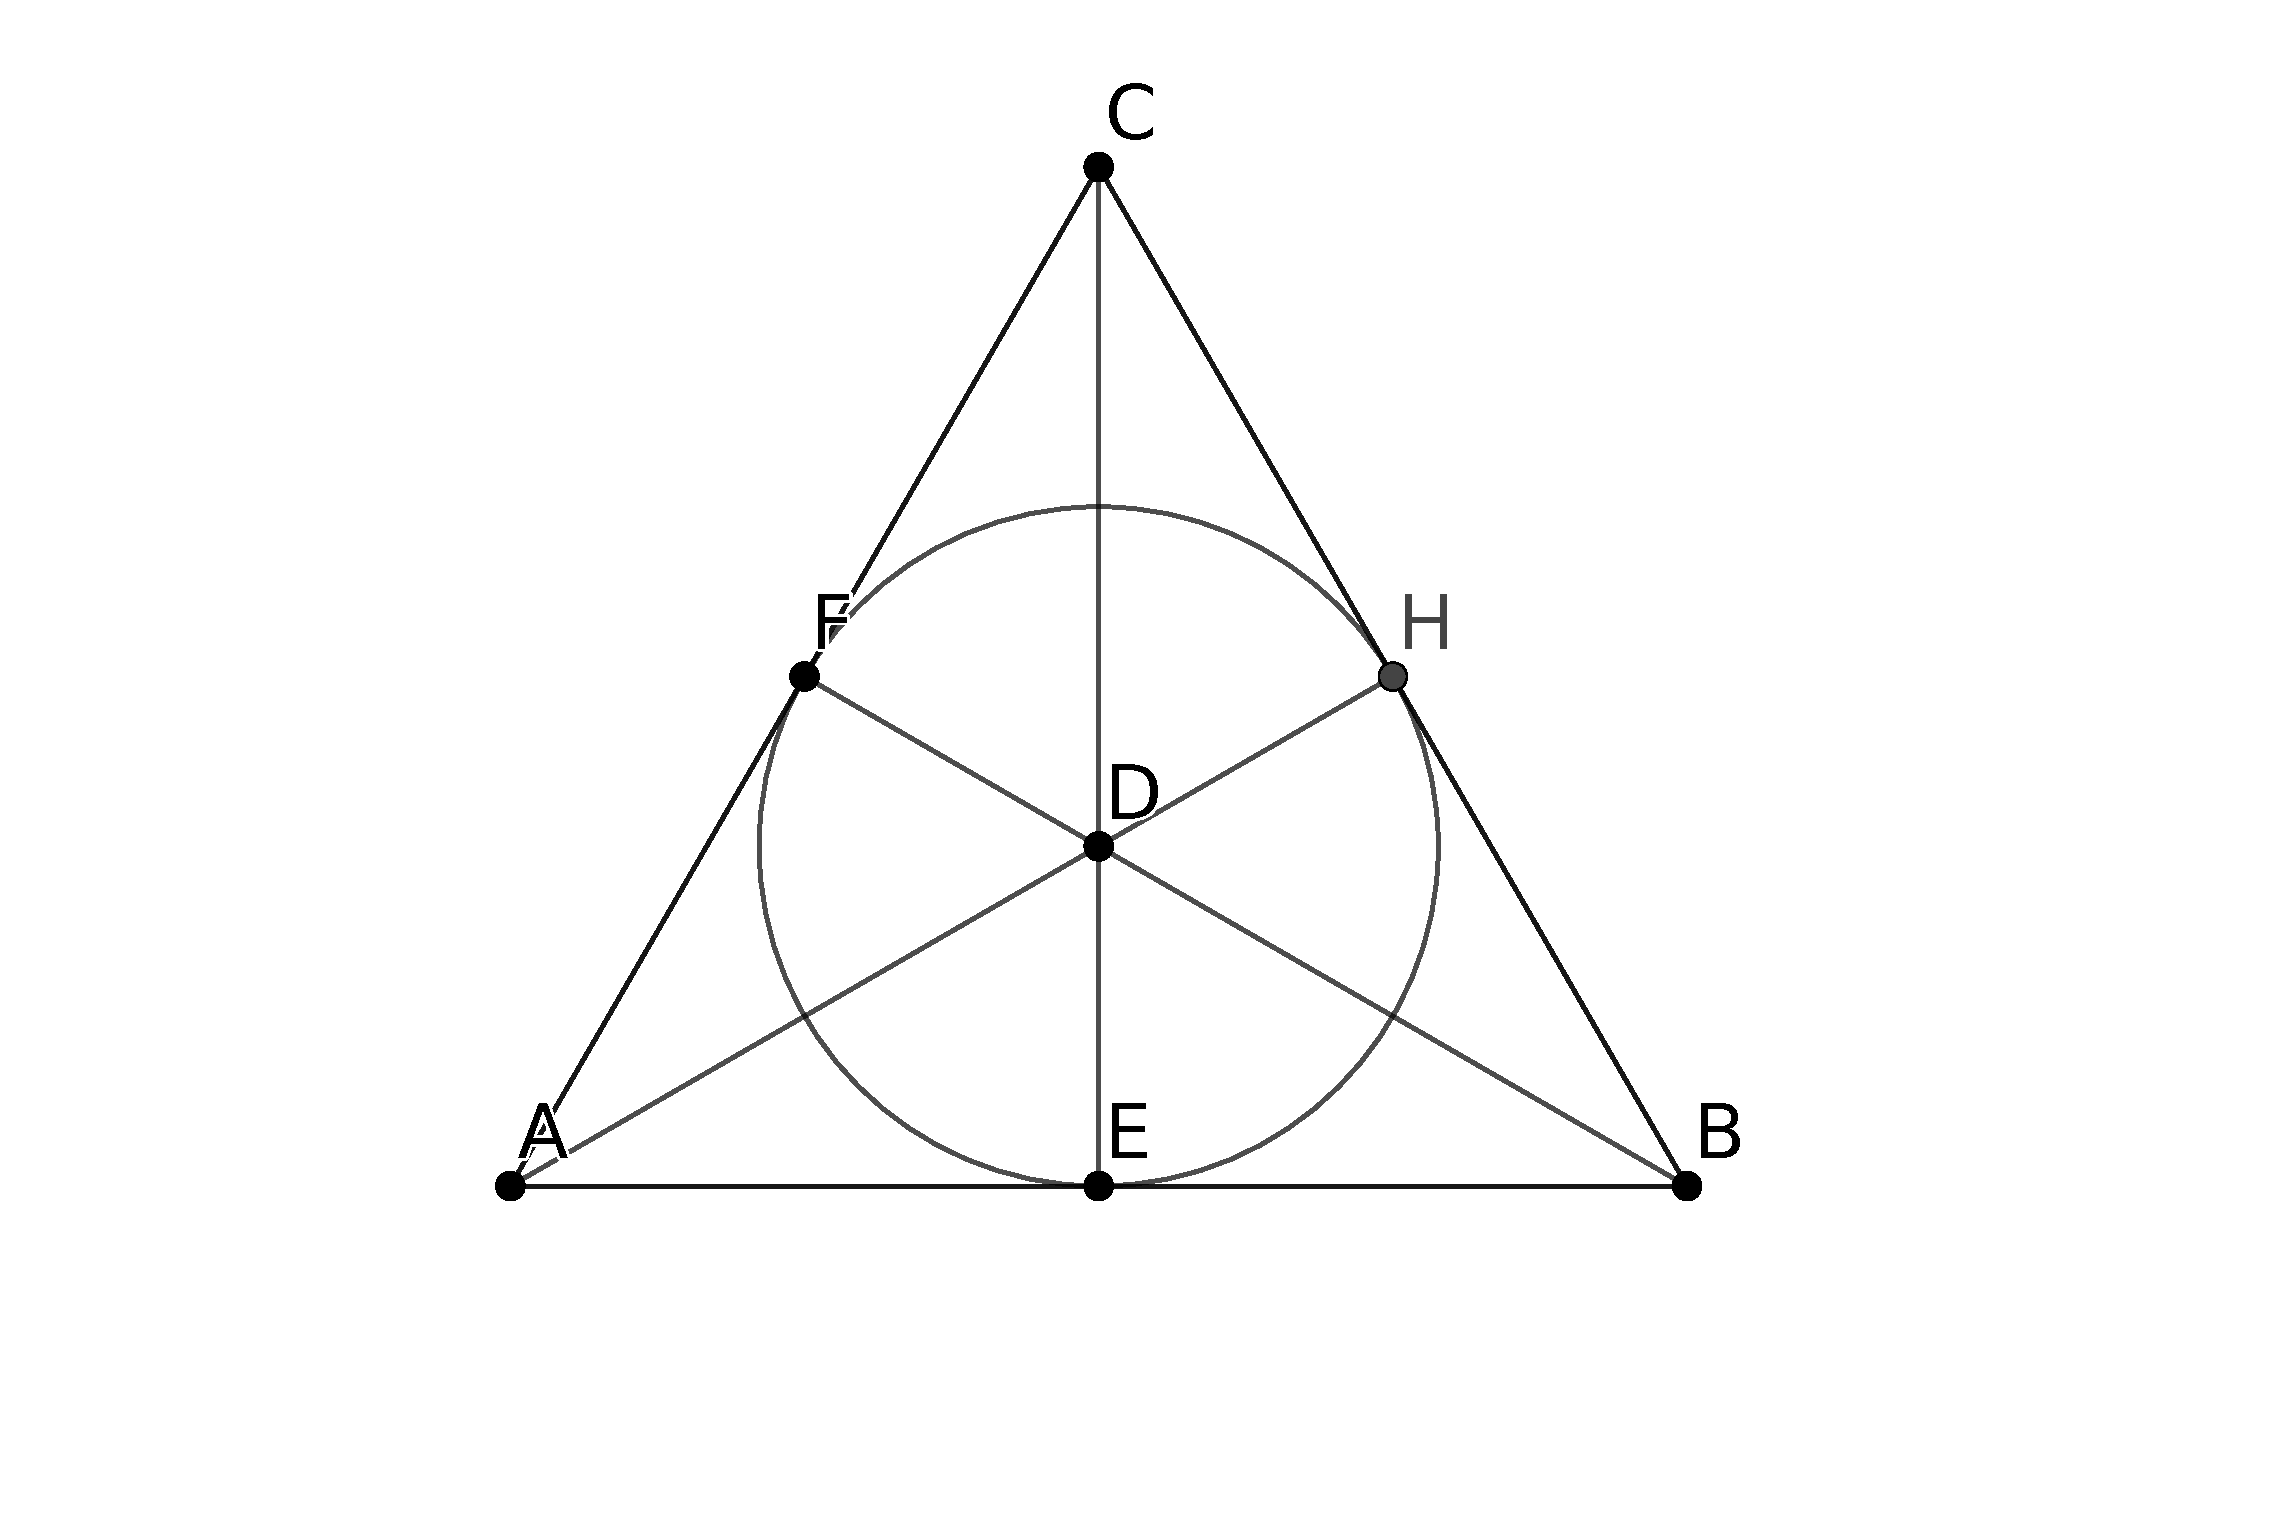
\includegraphics[scale=0.3]{fano2.pdf}
    \caption{Fanova projektívna rovina}
    \label{fig:fano_fpp}
\end{figure}


\begin{definition}
\label{def:m_fano}
Nech $\pi_F = (X, \mathcal{B}, \in)$ je Fanova projektívna rovina (viď obrázok \ref{fig:fano_fpp}).
Nech množina $\mathcal{N}$ obsahuje všetky podmnožiny $X$ mohutnosti najviac dva a také trojice bodov, ktoré neležia na jednej priamke.
Potom $(X, \mathcal{N})$ je Fanov matroid a označuje sa $\mathcal{F}$.
\end{definition}

\begin{exercise}
Overte, či definícia \ref{def:m_fano} spĺňa podmienky z definície matroidu.
\end{exercise}


\begin{definition}
Nech $X:=\set{1, \ldots, n}$, $\mathcal{N}:=\set{A ~|~ A \subseteq X \wedge \ssize{A} \leq k}$. Potom 
dvojica $U_k^n = (X, \mathcal{N})$ je matroid.
\end{definition}

\begin{theorem}
\label{th:m_unk}
$(U_k^n)^* = U_{n-k}^n$
\end{theorem}

\begin{theorem_hard}{(Charakterizácia tried matroidov)}
\begin{enumerate}
    \item matroid M je binárny $\Longleftrightarrow$ $U_2^4$ nie je minorom matroidu~M.
    \item matroid M je regulárny $\Longleftrightarrow$ $U_2^4$, $\mathcal{F}$, $\mathcal{F}^*$ nie sú minormi matroidu~M.
    \item matroid M je grafový $\Longleftrightarrow$ $U_2^4$, $\mathcal{F}$, $\mathcal{F}^*$, $M^*(K_{3,3})$, $M^*(K_{5})$ nie sú minormi matroidu~M.
    \item matroid M je kografový $\Longleftrightarrow$ $U_2^4$, $\mathcal{F}$, $\mathcal{F}^*$, $M(K_{3,3})$, $M(K_{5})$ nie sú minormi matroidu~M.
    \item matroid M je planárny $\Longleftrightarrow$ matroid M je grafový a kografový.
\end{enumerate}
\end{theorem_hard}


\section{Matroidové algoritmy}

\begin{definition}

Problém maximálnej množiny je trojica $(X, \mathcal{M}, c)$, kde 
$X = {x_1, \ldots, x_n}$ je množina objektov, 
$\mathcal{M} \subseteq \powerset(X)$ je množina prípustných riešení a $c: X \to \mathbb{R}^+ \cup \set{0}$
je cenová funkcia, rozšíriteľná na $\powerset(X)$, a to takým spôsobom: $\forall A \in \powerset(X): c(A) := \sum_{x_i \in A} c(x_i) $.
Riešením problému maximálnej množiny je množina $M^* \in \mathcal{M}$ s maximálnou cenou. Formálne,
$$M^* := \underset{M \in \mathcal{M}}{\arg\max}~c(M)$$

\end{definition}

\begin{definition}{(Pažravý algoritmus)}\\
Nech $(X, \mathcal{M}, c)$ je problém maximálnej množiny. Potom nasledovný algoritmus je pažravým algoritmom pre nájdenie riešenia
daného problému:
\begin{enumerate}
    \item $M_0 := \varnothing$
    \item $M_{i+1} := M_i \cup \set{x}$, ak $x$ spĺňa nasledovné podmienky:
    \begin{enumerate}
        \item $x \not\in M_i$
        \item $M_i \cup \set{x} \subseteq M' \in \mathcal{M}$ (t.j. existuje také $M' \in \mathcal{M}$)
        \item $x$ má spomedzi všetkých prvkov, ktoré spĺňajú predchádzajúce podmienky, maximálnu cenu $c(x)$
    \end{enumerate}
    \item Opakujeme krok 2. Ak $x$, vyhovujúce všetkým podmienkam z druhého kroku, neexistuje, tak algoritmus končí a odpoveďou je posledná množina $M_i$.
\end{enumerate}
\end{definition}

\begin{theorem}{(Vzťah matroidov a pažravých algoritmov)}\\
Nech $X$ je konečná množina, $\mathcal{M} \subseteq \powerset(X)$. Potom nasledujúce podmienky sú ekvivalentné:
\begin{enumerate}
    \item pre každé nezáporné ohodnotenie $c$ množiny $X$ pažravý algoritmus nájde optimálne riešenie
    \item existuje matroid na množine $X$ taký, že $\mathcal{M}$ je systémom báz daného matroidu 
\end{enumerate}
\end{theorem}
\todo[inline]{overit presne znenie vety (mnozina maximalnych na inkluziu pripustnych rieseni je systemom baz?)}
